\documentclass[letter, 10pts]{article}
\usepackage[monocolor]{../math232/ahsansabit}
\usepackage[]{float}
\usepackage{tikz}
\usepackage{tikz-3dplot}
\usepackage[outline]{contour} % glow around text
\usepackage{xcolor}
\usepackage{pdfpages}
\usepackage{physics}
\usepackage{multicol}
\title{Quantum Mechanics : : Homework 0X}
\author{Ahmed Saad Sabit, Rice University}
\date{\today}
\newcommand{\hb}{\hbar}
\newcommand{\U}{\uparrow}
\newcommand{\D}{\downarrow}
\usepackage[]{braket}
\begin{document}
\maketitle






























\section*{Problem 01} 
\subsection*{(a)} 
For the first particle in position $\theta = \Omega t$. 
\begin{align*}
\vec{F}_\text{cor} (\theta) &= - 2m \vec{\omega} \times \vec{v}(t) = - 2m \vec{\omega} \times  (\vec{\Omega} \times \vec{R}(t) )\\
&=
- 2 m (\omega \hat{z}) \times  
\left(
\Omega \vec{y} \times 
\left[
R \cos \theta \hat{x} + R \sin \theta \hat{z}
\right]
\right)
\\
&= 
- 2m \omega \hat{z} \times \left(
\Omega R \cos \theta(- \hat{z}) + \Omega R \sin  \theta (- \hat{x})
\right)
\\
&= 
2m \omega \hat{z} \times \left(
\Omega R \cos \theta\hat{z} + \Omega R \sin  \theta  \hat{x}
\right)
\\
&= 
2 m \omega \Omega R (- \hat{y})
\\
&= 
- 2 m \omega \Omega R \sin (\theta)\hat{y}
\end{align*}

For the second particle is $\vec{F}_\text{cor}(\theta + \pi )$.  $\vec{F}_\text{cor} = 2 m \omega \Omega R \sin(\omega) \hat{y}$








\subsection*{(b)} 
\begin{align*}
\vec{\tau} &= 
\vec{R}_1 \times \vec{F}_1 + \vec{R}_2 \times  \vec{F}_2  
\\
&= 
\left(
R \cos \theta \hat{x} + R \sin \theta \hat{z}
\right) \times  (- 2m \omega \Omega R \sin \theta \hat{y})
+ \left(
 -R \cos \theta \hat{x} - R \sin \theta \hat{z}
\right) \times  (2m \omega \Omega R \sin \theta \hat{y})
\\
&= 
\left[
	(-2 m \omega \Omega R^2 ) \left(\cos \theta \hat{x} \times \sin \theta \hat{y} + \sin \theta \hat{z} \times  \sin \theta \hat{y}\right)
\right]
\\
&= 
2 \left[
	(-2 m \omega \Omega R^2 ) \left(- \cos \theta \sin \theta \hat{z}   + \sin ^2 \theta \hat{x}\right)
\right] \\  
&= 
	4 m \omega \Omega R^2  \left(\cos \theta \sin \theta \hat{z}   - \sin ^2 \theta \hat{x}\right)
\end{align*}













\subsection*{(c)} 
\begin{align*}
	\vec{\tau} &= 4 m \omega \Omega R^2 \left(\cos \theta\sin \theta \hat{z} - \sin ^2 \theta \hat{x} \right) \\
	\braket{ \vec{\tau}} 
		   &= \frac{\int_{0}^{T} \mathrm{d} t \,  4 m \omega \Omega R^2 
		   \left(\cos (\Omega t) \sin (\Omega t) \hat{z} - \sin ^2 (\Omega t) \hat{x} \right)}{\int_{0}^{T } \mathrm{d} t }  \\ 
		   &= \frac{\int_{0}^{T} \mathrm{d} t \,  4 m \omega \Omega R^2 
		   \left(\cos (\Omega t) \sin (\Omega t) \hat{z} - \sin ^2 (\Omega t) \hat{x} \right)}{\int_{0}^{T } \mathrm{d} t } 
		   \tag{$T = 2 \pi / \Omega$ } \\ 
&= 
{4 m \omega \Omega R^2} 
\frac{\left[ \hat{z}
\int_{0}^{T} \mathrm{d} t \, \cos(\Omega t) \sin(\Omega t)  - 
\hat{x} \int_{0}^{T} \mathrm{d} t \, \sin ^2 (\Omega t)  
\right]}{2 \pi / \Omega} 
\\
&= 
4 m \omega \Omega R^2 \left(
- \frac{1}{2} \hat{x}
\right)
\\
&= 
-2 m \omega \Omega R^2 
\hat{x}
\\
\end{align*}









\subsection*{(d)} 


















\section*{Problem 02}
\subsection*{(a)}
\begin{align*}
\frac{\mathrm{d} }{\mathrm{d} t} \left(\vec{A} \cdot  \vec{B}\right)_\text{fix} &= 
\left(
\frac{\mathrm{d} \vec{A}}{\mathrm{d} t} \cdot \vec{B}
\right)_\text{fix} + 
\left(
\vec{A} \cdot  \frac{\mathrm{d} \vec{B}}{\mathrm{d} t}
\right)_\text{fix}
\\
\left(
\frac{\mathrm{d} \vec{A}}{\mathrm{d} t} \right)_\text{fix} 
&= 
\left(\frac{\mathrm{d} \vec{A}}{\mathrm{d} t}\right)_\text{rot}+ \vec{\omega} \times \vec{A} \\
\left(
\frac{\mathrm{d} \vec{B}}{\mathrm{d} t} \right)_\text{fix} 
&= 
\left(\frac{\mathrm{d} \vec{B}}{\mathrm{d} t}\right)_\text{rot}+ \vec{\omega} \times \vec{B} \\ 
\\\implies
\frac{\mathrm{d} }{\mathrm{d} t} \left(\vec{A} \cdot  \vec{B}\right)_\text{fix} = 
\left(
\frac{\mathrm{d} \vec{A}}{\mathrm{d} t} \cdot \vec{B}
\right)_\text{fix} + 
\left(
\vec{A} \cdot  \frac{\mathrm{d} \vec{B}}{\mathrm{d} t}
\right)_\text{fix} 
&= \left[
\left(\frac{\mathrm{d} \vec{A}}{\mathrm{d} t}\right)_\text{rot}+ \vec{\omega} \times \vec{A}
\right]\cdot \vec{B}
+\left[
\left(\frac{\mathrm{d} \vec{B}}{\mathrm{d} t}\right)_\text{rot}+ \vec{\omega} \times \vec{B}
\right]\cdot \vec{A}\\
&= 
\left(\frac{\mathrm{d} A}{\mathrm{d} t}\right)_\text{rot} \cdot \vec{B} + 
\left(\frac{\mathrm{d} B}{\mathrm{d} t}\right)_\text{rot} \cdot \vec{A} + 
\left[
	(\vec{\omega} \times \vec{A}) \cdot \vec{B} + (\vec{\omega} \times \vec{B}) \cdot \vec{A}
\right] \tag{check appendix for why third term is zero}
\\
&= 
\left(\frac{\mathrm{d} A}{\mathrm{d} t}\right)_\text{rot} \cdot \vec{B} + 
\left(\frac{\mathrm{d} B}{\mathrm{d} t}\right)_\text{rot} \cdot \vec{A} 
\\
&= 
\frac{\mathrm{d} }{\mathrm{d} t} 
\left(
\vec{A} \cdot \vec{B}\right)_\text{rot}\\
\end{align*}

\subsection*{(b)}
Recycling what we had above, using $\vec{C} = \vec{A} \times \vec{B}$ 
\begin{align*}
	\left( \frac{d\vec{C}}{dt} \right)_{\text{fixed}} &= \left( \left( \frac{d\vec{A}}{dt} \right)_{\text{rotating}} + \vec{\omega} \times \vec{A} \right) \times \vec{B} + \vec{A} \times \left( \left( \frac{d\vec{B}}{dt} \right)_{\text{rotating}} + \vec{\omega} \times \vec{B} \right).
\\
							  &= \left( \frac{d\vec{A}}{dt} \right)_{\text{rotating}} \times \vec{B} + (\vec{\omega} \times \vec{A}) \times \vec{B} + \vec{A} \times \left( \frac{d\vec{B}}{dt} \right)_{\text{rotating}} + \vec{A} \times (\vec{\omega} \times \vec{B})
							  \\ &= 
							  \left[ \left( \frac{d\vec{A}}{dt} \right)_{\text{rotating}} \times \vec{B} + \vec{A} \times \left( \frac{d\vec{B}}{dt} \right)_{\text{rotating}} \right] + \left[ (\vec{\omega} \times \vec{A}) \times \vec{B} + \vec{A} \times (\vec{\omega} \times \vec{B}) \right]
\\
							     &= \left( \frac{d\vec{A}}{dt} \right)_{\text{rotating}} \times \vec{B} + \vec{A} \times \left( \frac{d\vec{B}}{dt} \right)_{\text{rotating}} + \vec{\omega} \times (\vec{A} \times \vec{B}) \tag{check appendix for proof}\\
							     &= \left( \frac{\mathrm{d} }{\mathrm{d} t} \vec{A} \times \vec{B} \right)_{\text{rotating}} + \vec{\omega} \times (\vec{A} \times \vec{B}) \\ 
							     &= 
							     \left(\frac{\mathrm{d} }{\mathrm{d} t} \vec{C}\right)_\text{rotating} + \vec{\omega} \times \vec{C}\\
\end{align*}
So vectors abide by the laws of rotation. 







\section*{Problem 03}
In a  steady rotational frame, intuitively speaking rough - the position dependent force is \emph{Centrifugal Force} and velocity dependent forces are  \emph{Coriolis Force}.  

\subsection*{(a)}
Consider no force of magnetic field now. Then all the fictitious forces
\[
\vec{F}  = m \ddot{\vec{r}}= - 2m  \vec{\omega} \times \vec{v} 
- m \vec{\omega} \times (\vec{\omega} \times \vec{r})
\] 
Now including magnetic force
\[\boxed{
\vec{F}  = m \ddot{\vec{r}}= - 2m  \vec{\omega} \times \vec{v} 
- m \vec{\omega} \times (\vec{\omega} \times \vec{r})
- q \vec{v} \times \vec{B}
} \] 

\subsection*{(b)} 
Substituting $q = 2 m \omega / B$ yields 
\begin{align*}
	\vec{F} &= - 2m \omega v 
\Biggr[ 
\hat{z} \times \hat{v}
\Biggr]
- m \omega^2 r \Biggr[ \hat{z} \times (\hat{z} \times \hat{r} ) \Biggr]- 
\left(
\frac{2 m \omega}{B}
\right)v B \Biggr[\hat{v} \times \hat{z}\Biggr] \\
	&= - 2m \omega v 
\Biggr[ 
\hat{z} \times \hat{v}
\Biggr]
- m \omega^2 r \Biggr[ \hat{z} \times (\hat{z} \times \hat{r} ) \Biggr]- 
2 m \omega v  \Biggr[\hat{v} \times \hat{z}\Biggr] \\
	&= 
- m \omega^2 r \Biggr[ \hat{z} \times (\hat{z} \times \hat{r} ) \Biggr] \\ &=
 m \omega^2 r \Biggr[ (\hat{z}\cdot \hat{z} ) \hat{r} \Biggr]
									\\ &= 
								 m \omega^2 \vec{r}
\end{align*}
This leaves us with 
\[
\ddot{\vec{r}} + \omega^2 \vec{r} = 0
\] 
This is a simple harmonic equation, Yippie! Please note that this equation holds in the rotational frame. 




\textbf{Details on shape: } Equilibrium is established at $r = 0$ hence establishing the center of the turntable to be the center. Two component solution 
\begin{align*}
	\ddot{x} + \omega^2 x &= 0  \implies x = x_0 \sin(\omega t + \phi_x)\\ 
	\ddot{y} + \omega^2 y &= 0 \implies y = y_0 \sin(\omega t + \phi_y)\\ 
\end{align*}
This is the very beautiful \emph{Lissayous Curves!}

\begin{figure}[H]
	\centering
	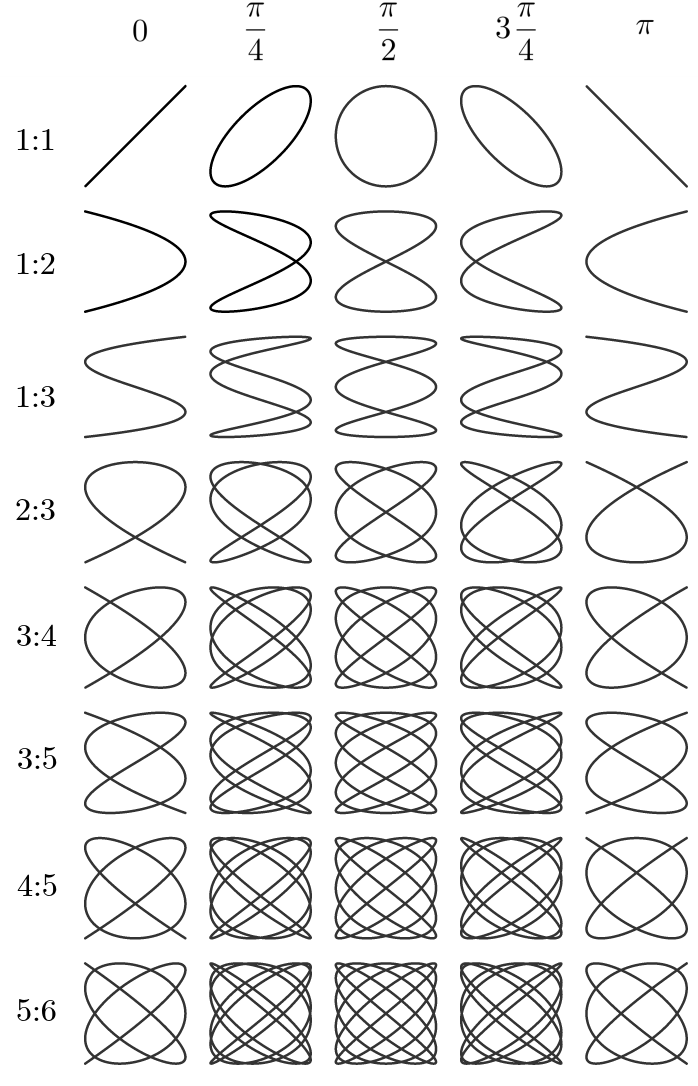
\includegraphics[width=0.4\textwidth]{./ss/9/1.png}
	\caption{Ratio of $x_0:y_0$ versus the phase difference $|\phi_x - \phi_y|$}
	\label{fig:-ss-9-1-png}
\end{figure}



\newpage
\subsection*{(c)}
For half as large $q$ we end up with 
\begin{align*}
	\vec{F}  &=  - 2m  \vec{\omega} \times \vec{v} 
- m \vec{\omega} \times (\vec{\omega} \times \vec{r})
- q \vec{v} \times \vec{B} \\ 
	 &= - 2m \omega v 
\Biggr[ 
\hat{z} \times \hat{v}
\Biggr]
- m \omega^2 r \Biggr[ \hat{z} \times (\hat{z} \times \hat{r} ) \Biggr]- 
\left(
q
\right)v B \Biggr[\hat{v} \times \hat{z}\Biggr] \\
		&= - 2m \omega v 
\Biggr[ 
\hat{z} \times \hat{v}
\Biggr]
- m \omega^2 r \Biggr[ \hat{z} \times (\hat{z} \times \hat{r} ) \Biggr]- 
\frac{1}{2}
\left(
\frac{2 m \omega}{B}
\right)v B \Biggr[\hat{v} \times \hat{z}\Biggr] \\
&= 
- 2m \omega v 
\left(
	[\hat{z} \times \hat{v} ] + \frac{1}{2} [\hat{v} \times \hat{z}] 
\right)- m \omega^2 \vec{r}
\\
&= 
- 2m \omega v 
\left(
	[\hat{z} \times \hat{v} ] - \frac{1}{2} [\hat{z} \times \hat{v}] 
\right)- m \omega^2 \vec{r}
\\
&= 
- 2m \omega v 
\left(
	 \frac{1}{2} [\hat{z} \times \hat{v}] 
\right)- m \omega^2 \vec{r}
\\
&= 
- m \omega v 
	[\hat{z} \times \hat{v}] 
- m \omega^2 \vec{r}
\\
\frac{\mathrm{d} \vec{v}}{\mathrm{d} t} &= 
- \omega v \left( \hat{z} \times  \hat{v} \right) - \omega^2 \vec{r}
\tag{NOTE: rotating frame derivative}
\\
\frac{\mathrm{d} \vec{v}}{\mathrm{d} t} &= - \vec{\omega} \times  \vec{v} - \omega^2 \vec{r} \\
\\
\end{align*}
The second derivative of a purely rotating vector $\vec{A}$ with $\vec{\Omega}$
\begin{align*}
	\frac{\mathrm{d} \vec{A}}{\mathrm{d} t} &= \vec{\Omega} \times \vec{A}\\
	\frac{\mathrm{d}^2 \vec{A}}{\mathrm{d} t^2} &=
\vec{\Omega}\times 	\left[\vec{\Omega} \times \vec{A}\right]\\
&=  - 
\Omega^2 \vec{A} 
\\
\end{align*}


%%
%
%
%
%
This is a derivative in the rotating frame, for an outside observer, 
\begin{align*}
\frac{\mathrm{d} \vec{v}}{\mathrm{d} t} + \vec{\omega} \times \vec{v} = \frac{\mathrm{d} \vec{v}}{\mathrm{d} t} \Biggr|_\text{lab} = \frac{\mathrm{d} ^2 \vec{r}}{\mathrm{d} t^2} = - \omega^2 \vec{r}
\end{align*}






\newpage
\section*{\((\vec{\omega} \times \vec{A}) \cdot \vec{B} = -\vec{A} \cdot (\vec{\omega} \times \vec{B})\)}

\[
\vec{\omega} = (\omega_x, \omega_y, \omega_z), \quad \vec{A} = (A_x, A_y, A_z), \quad \vec{B} = (B_x, B_y, B_z).
\]

\[
\vec{\omega} \times \vec{A} = 
\begin{vmatrix}
\hat{i} & \hat{j} & \hat{k} \\
\omega_x & \omega_y & \omega_z \\
A_x & A_y & A_z
\end{vmatrix}.
\]

\[
\vec{\omega} \times \vec{A} = \big( \omega_y A_z - \omega_z A_y \big)\hat{i} - \big( \omega_x A_z - \omega_z A_x \big)\hat{j} + \big( \omega_x A_y - \omega_y A_x \big)\hat{k}.
\]


\[
(\vec{\omega} \times \vec{A}) \cdot \vec{B} = (\omega_y A_z - \omega_z A_y)B_x + (-(\omega_x A_z - \omega_z A_x))B_y + (\omega_x A_y - \omega_y A_x)B_z.
\]

\[
= \omega_y A_z B_x - \omega_z A_y B_x - \omega_x A_z B_y + \omega_z A_x B_y + \omega_x A_y B_z - \omega_y A_x B_z.
\]

\[
\vec{\omega} \times \vec{B} = 
\begin{vmatrix}
\hat{i} & \hat{j} & \hat{k} \\
\omega_x & \omega_y & \omega_z \\
B_x & B_y & B_z
\end{vmatrix}.
\]

\[
\vec{\omega} \times \vec{B} = \big( \omega_y B_z - \omega_z B_y \big)\hat{i} - \big( \omega_x B_z - \omega_z B_x \big)\hat{j} + \big( \omega_x B_y - \omega_y B_x \big)\hat{k}.
\]


\[
-\vec{A} \cdot (\vec{\omega} \times \vec{B}) = -\left(A_x (\omega_y B_z - \omega_z B_y) + A_y (-(\omega_x B_z - \omega_z B_x)) + A_z (\omega_x B_y - \omega_y B_x)\right).
\]


\[
= \omega_y A_z B_x - \omega_z A_y B_x - \omega_x A_z B_y + \omega_z A_x B_y + \omega_x A_y B_z - \omega_y A_x B_z.
\]

Comparing the expanded expressions for
\[
(\vec{\omega} \times \vec{A}) \cdot \vec{B} \quad \text{and} \quad -\vec{A} \cdot (\vec{\omega} \times \vec{B}),
\]
we see they are identical. Therefore
\[
(\vec{\omega} \times \vec{A}) \cdot \vec{B} = -\vec{A} \cdot (\vec{\omega} \times \vec{B}).
\]


\section*{$(\vec{\omega} \times \vec{A} ) \times  \vec{B} + \vec{A} \times  (\vec{\omega} \times \vec{B})$}

\[
(\vec{\omega} \times \vec{A}) \times \vec{B} = \big((\vec{\omega} \times \vec{A}) \cdot \vec{B}\big) \vec{A} - \big((\vec{\omega} \times \vec{A}) \cdot \vec{A}\big) \vec{B}.
\]


\[
\vec{A} \times (\vec{\omega} \times \vec{B}) = \big(\vec{A} \cdot \vec{B}\big) \vec{\omega} - \big(\vec{A} \cdot \vec{\omega}\big) \vec{B}.
\]

\[
(\vec{\omega} \times \vec{A}) \times \vec{B} + \vec{A} \times (\vec{\omega} \times \vec{B}) = \vec{\omega} \times (\vec{A} \times \vec{B}).
\]
\end{document}
